\documentclass{article}
\setlength{\oddsidemargin}{0.25 in}
\setlength{\evensidemargin}{-0.25 in}
\setlength{\topmargin}{-0.6 in}
\setlength{\textwidth}{6.5 in}
\setlength{\textheight}{8.5 in}
\setlength{\headsep}{0.75 in}
\setlength{\parindent}{0 in}
\setlength{\parskip}{0.1 in}

% ===== PACKAGES =====
\usepackage{amsmath,amssymb}
\usepackage{color}
\usepackage{subfigure}
\usepackage{mdframed}
\usepackage{changepage}
\usepackage{graphicx}
\usepackage{hyperref}
\newmdenv[
  topline=false,
  bottomline=false,
  skipabove=\topsep,
  skipbelow=\topsep
]{siderules}
\renewcommand{\abstractname}{}


% ===== VARIABLES =====
\def \R{\mathbb{R}}
\def \Pr{\mathbb{P}}
\def \D{{\rm D}}
\def \N{{\rm N}}
\def \xx{{\boldsymbol{\rm x}}}
\def \y{{\rm y}}




% ===== HEADER BOX =====
\newcommand{\lecture}[2]{
\pagestyle{myheadings}
\thispagestyle{plain}
\newpage
\noindent
\begin{center}
\rule{\textwidth}{1.6pt}\vspace*{-\baselineskip}\vspace*{2pt} % Thick horizontal line
\rule{\textwidth}{0.4pt}\\[1\baselineskip] % Thin horizontal line
\vbox{\vspace{2mm}
\hbox to 6.28in { {\bf CS 760: Machine Learning} \hfill Spring 2022 }
\vspace{4mm}
\hbox to 6.28in { {\Large \hfill #1  \hfill} }
\vspace{4mm}
\hbox to 6.28in { {\scshape Authors:}  #2 \hfill }}
\vspace{-2mm}
\rule{\textwidth}{0.4pt}\vspace*{-\baselineskip}\vspace{3.2pt} % Thin horizontal line
\rule{\textwidth}{1.6pt}\\[\baselineskip] % Thick horizontal line
\end{center}
\vspace*{4mm}
}



% =============== DOCUMENT ===============
\graphicspath{ {./images} }
\begin{document}
\lecture{Final Project}{Ayushi Mishra, Neil Bhutada}

\begin{center}
{\Large {\sf \underline{\textbf{DO NOT POLLUTE!}} AVOID PRINTING, OR PRINT 2-SIDED MULTIPAGE.}}
\end{center}

\begin{abstract}
Opportunistic Cardiometabolic Screening is a process of collecting Computerized Tomography (CT) data for a pateint. CT scan collects a series of X-ray images for different parts of the body assisted in analyzing Bone, Fat, and Muscle measures, along with Aortic clarification and Liver fat of pateints (Mayo Foundation, p.1). Combining this CT data along with clinical data, such as BMI, Framingham Risk Score (FRS), Metabolic Syndrome etc. of several pateints helped us in predicting in the \emph{biological age} and \emph{number of days before death} of pateints. To compute the Biological age of a pateint we compared their CT and clinical data with other normal (or healthy) pateints within various age groups. For our analysis, we utilized two Machine learning models including Gradient Boosting Machine (GBM) and Weighted K-Nearest Neighbour (Weighted K-NN) to predict \emph{biological age} and \emph{number of days before death} of pateints. After our implementation, we came to a conclusion that incorporating clinical data along with CT data aided in improving our predictions for \emph{biological age} by $\sim{40}\%$ and \emph{number of days before death} by $\sim{16}\%$. Comparing the two models, we realized that Gradient Boosting Machine (GBM) performed better compared to Weighted K-Nearest Neighbour in our analysis to predict the \emph{biological age} and \emph{number of days before death} with and without clinical data by $\sim{33}\%$.
\end{abstract}

\section{Introduction}

During Opportunistic Cardiometabolic Screening, alot of the data goes unused after a preliminary analysis. Thus, in attempt to make the Opportunistic Cardiometabolic Screening data obtained more useful, we analyzed the CT scan data to predict the \emph{biological age} and \emph{number of days before death} of a patient. To predict the \emph{number of days before death} we used the patient's calculated \emph{biological age}. The way we predicted biological age was by comparing CT and clinical data of a pateint to other healthy/normal patients of various age groups. For example, a 50 year-old person may have a body (in our case CT and clinical data) similar to other 80 year-olds. 
  
Initially, to compute a patient's \emph{biological age} we filtered out the data to select healthy and alive patients based on various age groups solely using their CT data. The filtered data of healthly patients with their \emph{chronological age} was used as the training dataset to predict the biological age. After creating a model to predict a patient's \emph{biological age}, we used this model to predict the \emph{biological age} of all the dead people in the dataset. Then with the CT data scans and \emph{biological age} of all the dead people, we developed a model to predict the \emph{number of days before death}. 
Then we incorporated clinical data (such as BMI, Metabolic Syndrome, Tobacco consumption, etc.) about patients to further filter healthy and alive people to predict the \emph{biological age}. Similarly, we created another model to predict the \emph{number of days before death} that uses a patient's clinical data, CT data, and newly calculated \emph{biological age}.

\section{Related/Similar Work}

Automated CT biomarkers for opportunistic prediction of future cardiovascular events and mortality in an asymptomatic screening population: a retrospective cohort study' by Pickhardt et. al potentially showed how clinical data along with CT data can improve insights and a model's performance to predict clinical outcomes.

\section{Dataset Description}

The \emph{Opportunistic Cardiometabolic Screening} is owned by Perry Pickhardt (Department of Radiology, UWMadison). The dataset consists of 9223 records, such that each records in the dataset represents a unique pateint. In our report, we will be using the following features of the dataset for our analysis:

\underline{\textbf{Clinical Data}}
 
\textbf{Body Mass Index (BMI)} that determines whether a person has a healthy weight, \textbf{Body Mass Index greater than 30 (BMI \textgreater{30})} shows if a person has a BMI greater than 30 and no means that a person has lower than 30 BMI, \textbf{Age at Computerized Tomography (Age at CT)} consists of chronological age reported during the CT scan, \textbf{Tobacco} tells if a pateint consumes tobacco or not, \textbf{Framingham Risk Score (FRS 10-year risk (\%))} is used to estimate 10-yr risk of developing coronary heart disease, \textbf{Fracture Risk Assessment Score (FRAX 10y Fx Prob (Orange-w/ DXA))} shows a 10yr probability of fracture at the femoral neck or spine, \textbf{Fracture Risk Assessment Score for hip (FRAX 10y Hip Fx Prob (Orange-w/ DXA))} shows a 10yr probability of hip fracture, \textbf{Metabolic Syndrome (Met Sx)} tells if a patient has the syndrome or not.
  
\underline{\textbf{Computerized Tomography Data}}

\textbf{Bone measure/BMD (L1 HU)} measures the amount of bone mineral density, \textbf{TAT Area (cm2)} Total Adipose tissue, \textbf{VAT Area (cm2)} Visceral Adipose tissue, \textbf{SAT Area (cm2)} Subcutaneous Adipose tissue, \textbf{VAT/SAT Ratio} analyzes cardiometabolic risk, \textbf{Total Body Area EA (cm2)} of a pateint, \textbf{Muscle HU} tells muscle measure in Hounsfeild units, \textbf{Muscle Area (cm2)} muscle area measure in cm2, \textbf{Skeletal Muscle Index (L3 SMI (cm2/m2))} indicator of muscle depletion, \textbf{Aortic Calcification (AoCa Agatston)} measures calcium deposists on the aortic valve, \textbf{Liver Fat (Liver HU (Median))} measures extra fat stored in the liver in Hounsfeild units            
 
\underline{\textbf{Clinical Outcomes}}

 \textbf{Death (DEATH [d from CT])} consists of the number of days after the CT scan when the death of the pateint tool place.

\section{Approach}

\subsection{Preliminary Analysis}

We began our analysis by first looking at CT scan data to understand how these features are correlated with age at CT or number of days before death. We saw that none of the features among the CT scan data seems to be correlated with number of days before death. Moreover, we saw that age at CT is slightly correlated with Bone Mineral Density (L1 BMD HU). 

Since there is very little correlation, to further understand the data we performed UMAP - a non-linear dimensionality reduction method - to see if there were any significant clusters in the data. From a very careful observation of the plot in  Figure 1  we can see that many points nearby have similar \emph{number of days before death}. 

\begin{figure}
\centering
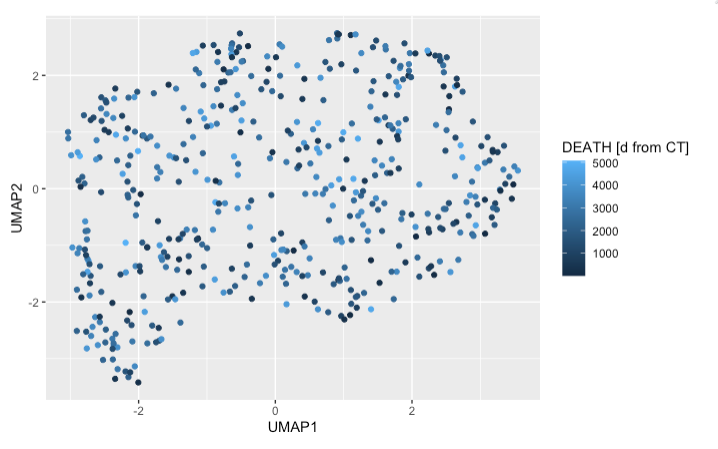
\includegraphics[width=10cm]{fig1-2}
\caption{UMAP of CT data}
\end{figure}

\subsection{Making predictions using only CT data}

\subsubsection{Pre-processing data to predict biological age}
\label{sec:two}
To filter out all the people who were healthy and alive, we assumed that all the outliers in the dataset were considered to be unhealthy. To proceed with our analysis, we performed Principal Component Analysis (PCA) on the above mentioned features of CT scan data to remove outliers. Thus, we filtered out the outliers from all the all principal components by only taking data that fell within $Q1 - 1.5 * IQR$ and $Q3 + 1.5 * IQR$, where Q1 represents 25th percentile value, Q3 represents 75th percentile value. After performing PCA, we realized that Aortic calcification and Bone Mineral Density (L1 BMD HU) still had some outliers. So, we again captured the data that fell within $Q1 - 1.5 * IQR$ and $Q3 + 1.5 * IQR$ for these features. 


\subsubsection{Model description for predicting biological age}
\label{sec:one}
To predict biological age, we used two models - Weighted-KNN and Gradient Boosting Machine (GBM)

Based on our definition of biological age defined above, our model has to look for patients with similar data (CT data scans, clinical data) and calculate their biological age. Furthermore, the model should give more importance to neighbouring data points. Hence, for predicting biological age we used Weighted-KNN as one option. 

\begin{figure}[h]
\centering
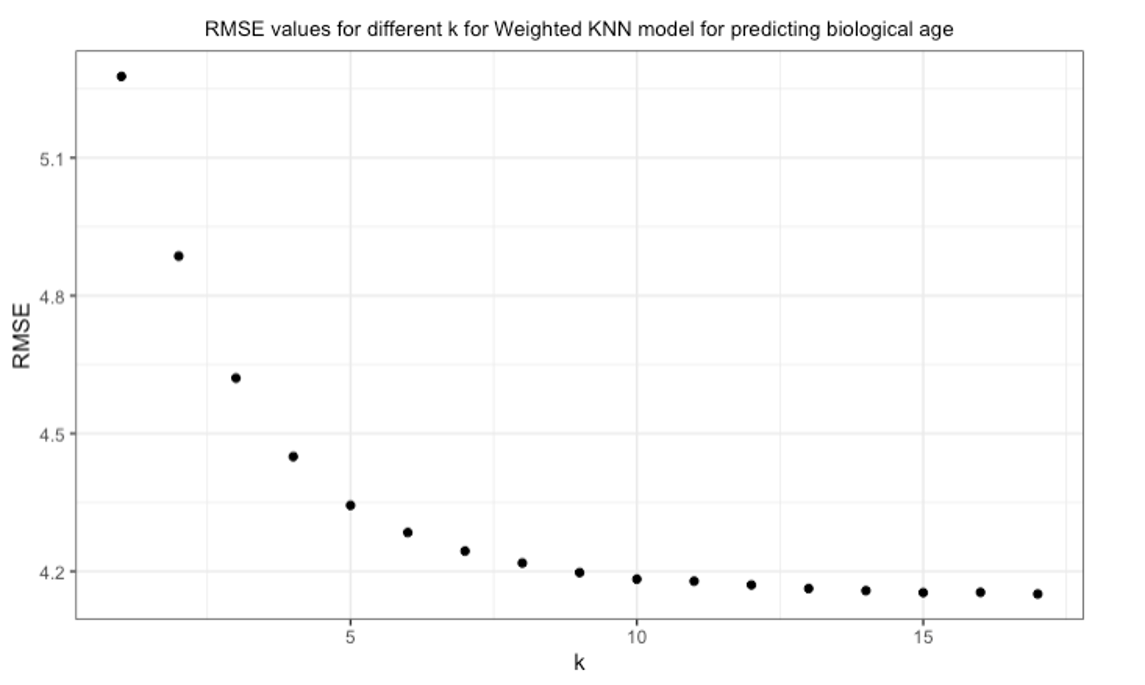
\includegraphics[width=10cm]{fig1-3}
\caption{RMSE for different values of k}
\end{figure}

We implemented Weighted-KNN using the "train.kknn" function in the "kknn" library. The "train.kknn" performs leave one out cross-validation and finds an optimal value of "k" if "kmax" is specified. From Figure 2, the optimal value of "k" seemed to be around 15. Weights are assigned to different neighbours based on the distance from the new observation and the kernel passed. The kernel here means the probability density function. According to the pseudo code, the weights are first normalized  and are between [$10^{-6}$, $1 - 10^{-6}$]. 


\begin{verbatim}
 W <- D/maxdist
 W <- pmin(W, 1 - (1e-06))
 W <- pmax(W, 1e-06)
\end{verbatim}
 
Now, the weights are further manipuated based on the kernel specified by the user. In our project, the "triangular" kernel gave us the optimal model. The following is the psuedo code for the manipulating the weights when the kernel is "triangular" : 

\begin{verbatim}
if (kernel == "triangular") 
        W <- 1 - W
\end{verbatim}

        
Eventually, the weights are then fitted by first computing the sum of the products of each weight with each observed value in the neighbour and then dividing by the sum of weights:

\begin{verbatim}
fit <- rowSums(W * CL)/pmax(rowSums(W), 1e-06)
\end{verbatim}

(Seinen, para. 1-3)

Based on our preliminary analysis, we also thought of using a model that is powerful enough to find hidden and complicated patterns. Hence, we decided to create a GBM model to predict the biological age. 

We implemented H2O's GBM, a forward-learning ensemble method used for predictive analysis, by utilizing its following functions:

\hspace*{10mm}• Mean squared error as the loss function

\hspace*{10mm}• Stochastic gradient boosting by the use of column and row sampling


GBM within H2O obtains its predictive results in two steps - 

\hspace*{10mm}1) Minimizing the model's loss function by utilizing the gradients.

\hspace*{10mm}2) Additively improves weaker models to increase the accuracy of predictions.

The Gradient Boosting Algorithm works in the following ways:

It begins by taking every row measurement and its corresponding response variable as input. It also takes in a differentiable loss function to evaluate our predictions. To predict biological age, we utilized Mean Squared error as our loss function.

\hspace*{10mm}$\text { Data }\left\{\left(x_{i}, y_{i}\right)\right\}_{i=1}^{n}, \text { and a differentiable Loss Function } L\left(y_{i}, F(x)\right)$

Then, we begin with our Step 1, 

\hspace*{10mm}Step 1: Initialize model with a constant value: $F_{0}(x)=\underset{\gamma}{\operatorname{argmin}} \sum_{i=1}^{n} L\left(y_{i}, \gamma\right)$

Here,  $L(y_{i}, \gamma)$ defines the loss function. In our case, $y_{i}$ represents the \emph{Age at CT} and $\gamma$ represents the predicted \emph{Biological age}. In this case, we find the predicted value that minimizes the loss function, i.e. Mean Squared error. We can find such $\gamma$ by simply taking the gradient. It is observed that the $\gamma$ that minimized $F_{0}(x)=\underset{\gamma}{\operatorname{argmin}} \sum_{i=1}^{n} L(y_{i}, \gamma)$ is the average of all the response values. Hence, $F_{0}(x)$ will just be a leaf that predicts each row as the same. 

Now, we will loop M times to create M trees. 

\hspace*{10mm}Step 2: for $m=1$ to $M$ :

In part A of Step 2, we just take the derivative of loss function with respect to the predicted value. Here, $y_{i}$ is the Age at CT and $F(x_{i}$ is the predicted biological age. On simplifying this term, we observe that $r_{i m}$ is equal to residual (Observed - Predicted). We can calculate $r_{i m}$ for each sample by plugging in $F(x)=F_{m-1}(x)$. 

\hspace*{10mm}$\text { (A) Compute } r_{i m}=-\left[\frac{\partial L\left(y_{i}, F\left(x_{i}\right)\right)}{\partial F\left(x_{i}\right)}\right]_{F(x)=F_{m-1}(x)} \text { for } i=1, \ldots, n$

In part B of Step 2, we will be building a regression tree to predict the residuals. The terminal regions $R_{j m}$, for $j=1 \ldots J_{m}$ are just the leaves of the regression tree.

\hspace*{10mm}(B) Fit a regression tree to the $r_{i m}$ values and create terminal regions $R_{j m}$, for $j=1 \ldots J_{m}$

In part C of Step 2, we compute output for each $j^{th}$ leaf in the tree such that it minimizes the summation mentioned below. In this case, the loss function also takes into account of the previous prediction ($F_{m-1}\left(x_{i}\right)$). Also, $x_{i}$ defines the records that fall within a particular leaf. The output of each leaf is the average of the outputs of all records that fall in that leaf.

\hspace*{10mm}(C) For $j=1 \ldots J_{m}$ compute $\gamma_{j m}=\underset{\gamma}{\operatorname{argmin}} \sum_{x_{i} \in R_{i j}} L\left(y_{i}, F_{m-1}\left(x_{i}\right)+\gamma\right)$

In part D of Step 2, we will make new prediction for each sample by utilizing the prediction of last step. In this step, we also use the learning rate to reduce the affect of each tree on the final prediction.

\hspace*{10mm}$\text { (D) Update } F_{m}(x)=F_{m-1}(x)+\nu \sum^{J_{m}} \gamma_{j m} I\left(x \in R_{j m}\right)$

Finally, output the result in the end. 

\hspace*{10mm}Step 3: Output $F_{M}(x)$

(Hastie et. al, 2001, p.339)

To optimize hyper-paramters such as number of trees, sample rate, etc. in the GBM, we used grids. To predict the biological age with only CT data, the GBM model was as followed:

\begin{verbatim}
h2o.gbm(2:12, 1, train, nfolds = 5, ntrees = 49,fold_assignment = "Modulo", score_tree_interval = 5, 
max_depth = 3,min_rows = 1, sample_rate = 0.9, col_sample_rate = 0.7, max_abs_leafnode_pred = 100)
\end{verbatim}



\subsubsection{Pre-processing data to predict death using CT data}

To decrease the variance of the reponse variable, i.e., 'Days Before Death', we converted this term into years by dividing the values by 365. Further more, in attempt to make the distribution non-uniform and less random, we took the log of the response variable.

\subsubsection{Model description for predicting number of days before death}

We again used Weighted K-NN and GBM to predict death using the CT scan data and newly computed biological age from the models mentioned above. To understand the underlying algorithms of Weighted K-NN and GBM please refer to \hyperref[sec:one]{section 4.2.2}. 

Using similar methods mentioned in \hyperref[sec:one]{section 4.2.2}, the optimal value of "k" was 18, and the "kernel" used was "rectangular." When the "kernel" is "rectangular", it implies that no weights have been added and unweighted K-NN is used.  

Likewise,to obtain optimal parameters we used Grids. The model parameters were:
\begin{verbatim}
h2o.gbm(c(1:2, 4:15), 3, train, nfolds = 5, ntrees = 24, max_depth = 3, sample_rate = 0.6,
col_sample_rate = 0.7,col_sample_rate_per_tree = 0.4)
\end{verbatim}

\subsection{Making predictions using CT and Clinical Data}

\subsubsection{Pre-processing data to predict biological age with clinical data}
The pre-processing concept was similar to \hyperref[sec:two]{section 4.2.1}. To filter out healthy people we only considered patients that had a BMI lesser than 30, consumed no tobacco, had a FRS 10-year risk score lesser than 0.19 (Bosomworth, 2011, para-6), and did not have any Metabollic synodrome. We removed outliers in FRAX scores and Aortic Calcification for each age group.

\subsubsection{Predicting biological age with CT and clinical data}

We used Weighted K-NN and GBM to predict the biological age using CT, clinical data. To understand the underlying algorithms of Weighted K-NN and GBM please refer to \hyperref[sec:one]{section 4.2.2}. The Weighted K-NN model for predicting biolgical age had "k" equal to 7 and the "kernel" set to "triangular." Similarly, the optimal parameters for the GBM model was: 

\begin{verbatim}
h2o.gbm(c(1, 3:16), 2, train, sample_rate = 0.8, col_sample_rate = 0.8, 
ntrees = 44, max_depth = 10, nfolds = 5, max_abs_leafnode_pred = 90)
\end{verbatim}

\subsubsection{Predicting death with CT and clinical data}

We used Weighted K-NN and GBM to predict death using CT, Clinical Data, and newly computed biological age in the section above. To understand the underlying algorithms of Weighted K-NN and GBM please refer to \hyperref[sec:one]{section 4.2.2}. The parameters for Weighted K-NN were "k" equal to 23 and the optimial kernel found was "gaussian". The psuedo code for the "gaussian" kernel is:

\begin{verbatim}
if (kernel == "gaussian") {
        alpha = 1/(2 * (k + 1)) #Computes significane level
        qua = abs(qnorm(alpha)) #Finds quantile, or point in gaussian curve to represent alpha
        W = W * qua #Scale weights with "qua" 
        W = dnorm(W, sd = 1) #Find probability density
    }
\end{verbatim}

(Seinen, para. 1-3)

A significance value "alpha" is found based on the number of neighbours "k" used. Then, we find a point in the gaussian distribution representing "alpha" - here called as "qua". We scale the weights by then multplying them with "qua". Then the new weights are equal to the probability density of the scaled weights. 

The optimal parameters for the GBM to predict death found using grids were:

\begin{verbatim}
h2o.gbm(c(1:2, 4:21), 3, train, sample_rate = 0.6, col_sample_rate = 0.7, ntrees =23, 
max_depth = 8, min_split_improvement = 0.0001, score_tree_interval = 5, nfolds = 10)
\end{verbatim}

\section{Results}

\subsection{Predicting Biological Age}
We initiated our experiment to predict \emph{Biological age} using the Weighted KNN model on CT scan data. Using this model, we made predictions on how well it estimates the \emph{biological age} of healthy people. With CT data only, the model's Root Mean Squared Error value came out to be \textbf{4.19 years}. After incorporating clinical data with CT data, we created the second model to predict \emph{biological age} and the RMSE score dropped down to \textbf{2.6 years}. 

Similarly, we predicted \emph{biological age} using GBM. Using the CT data of healthy and alive people as training data, we created the GBM model which predicted the \emph{biological age} with a RMSE of \textbf{3.28 years}. After incorporating clinical data with CT data, we created the second GBM model to predict \emph{biological age} and observed that the RMSE score dropped down to \textbf{2.088 years}.

Figure 3 shows comparisons between the performance of Weighted K-NN and GBM models that were obtained after incorporating clinical data.

\begin{figure}[h]
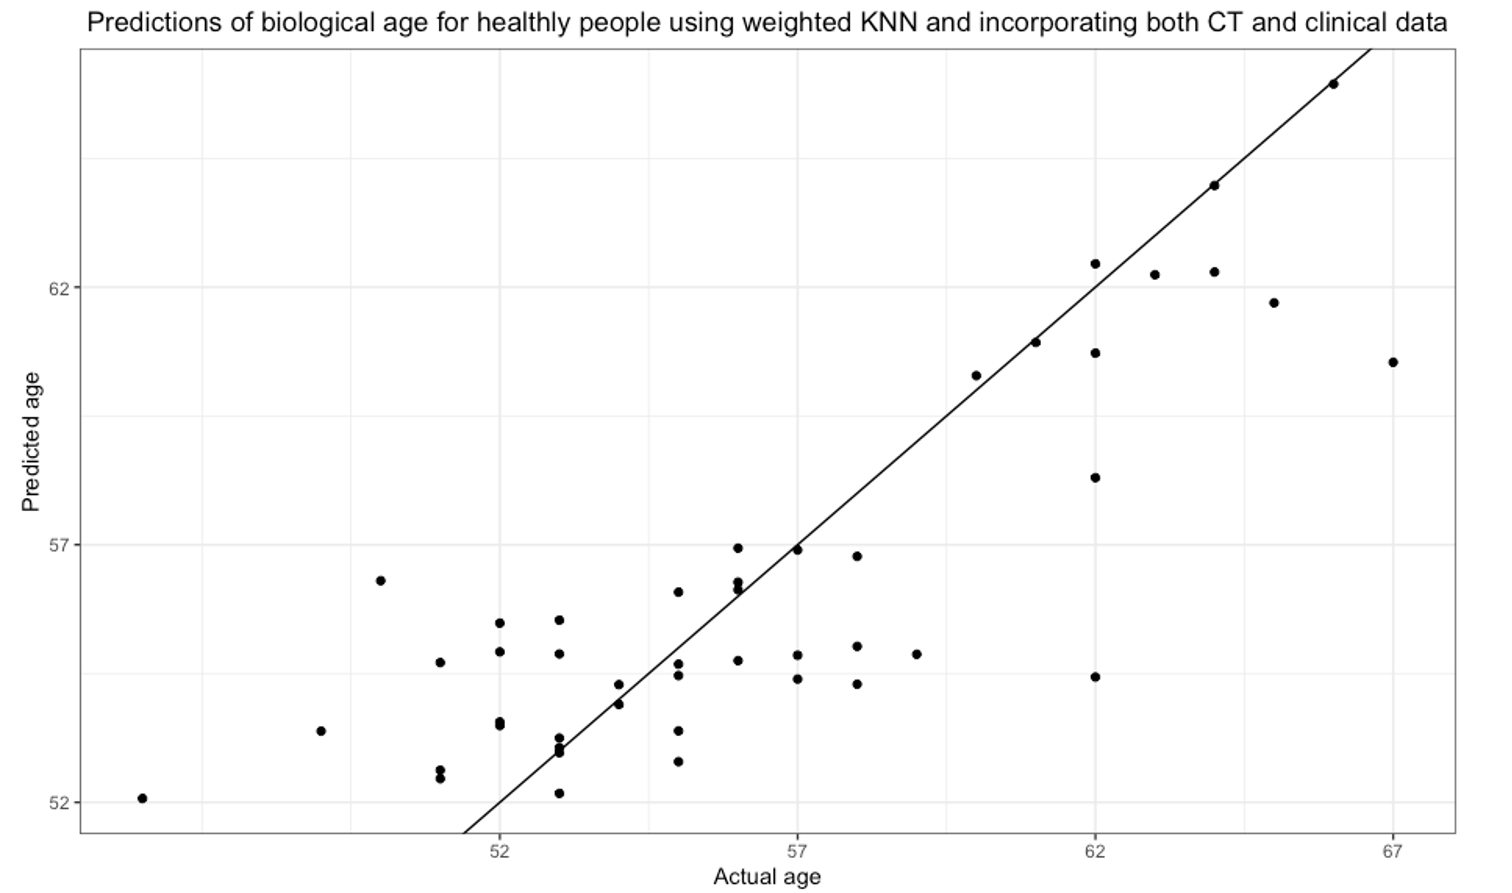
\includegraphics[height=4cm]{fig1-5}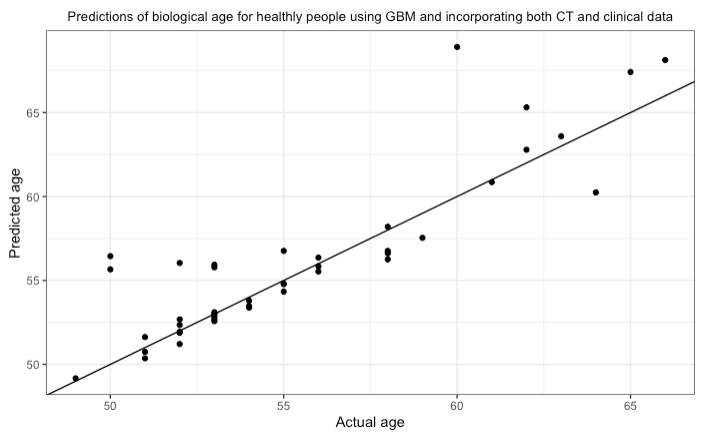
\includegraphics[height=4cm]{fig1-7}
\caption{Comparing Biological Age predictions between Weighted K-NN and GBM}
\end{figure}

\subsection{Predicting Death}

When using only the CT data and predicted biological age, the Weighted K-NN model gives a RMSE of around \textbf{3.12 years}. On the other hand, the GBM model gives a RMSE of around \textbf{2.7 years}. Furthermore, the GBM recognizes that the Biological Age is the second most important feature to predict death; however, the GBM considers Muscle HU to be the most important feature to predict death. 

Similarly, when incorporating clinical data, the weighted K-NN model gives a RMSE of around \textbf{2.4 years}. Likewise, the GBM models gives a RMSE of around \textbf{1.9 years}. Although Muscle HU and Biological Age seems to be the most important features to predict death, but FRAX scores have become the third most important feature.

From the UMAP visualizations in Figure 4 we can see how our best model, i.e, GBM with clinical data makes predictions that are similar in nature to the actual data

\begin{figure}[h]
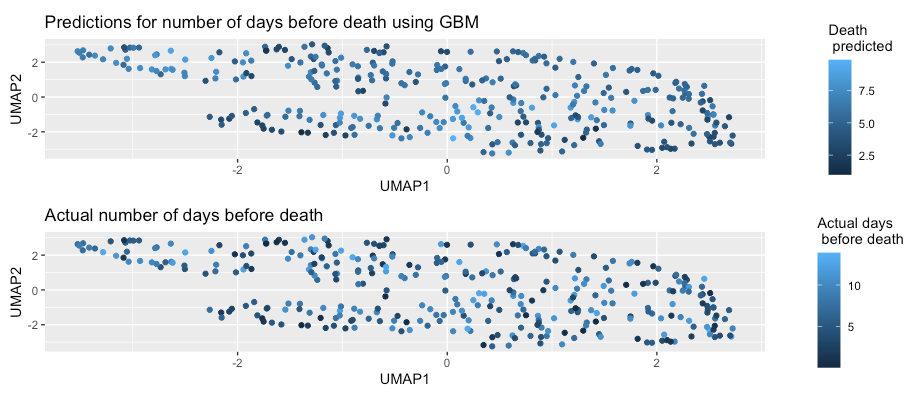
\includegraphics[height = 8cm]{fig1-11}
\caption{Comparing death predictions made by the best model with actual dataset}
\end{figure}



\section{Future Work}

To improve the Accuracy model, we could probably use a Stacked Ensemble with multiple GBMs, Random Forests, and Deep Learning models. We could perform Hypothesis testing on varibles such as Tobacco against death to verify or understand why it was not the most important feature. We could receive more data about healthy patients to improve the biological age predictions.

\pagebreak

\section{References}

Seinen, D. (n.d.). Weighted K-nearest neighbors and R kknn package. Stack Overflow. Retrieved May 12, 2022, from https://stackoverflow.com/questions/65654487/weighted-k-nearest-neighbors-and-r-kknn-package 


Bosomworth, N. J. (2011, April). Practical use of the Framingham Risk Score in Primary Prevention: Canadian Perspective. Canadian family physician Medecin de famille canadien. Retrieved May 12, 2022, from https://www.ncbi.nlm.nih.gov/pmc/articles/PMC3076470/ 


Hastie, Trevor, Robert Tibshirani, and J Jerome H Friedman. . (2001). In The Elements of Statistical Learning. (Vol. 1, p. 399). essay, Springer New York. 


Mayo Foundation for Medical Education and Research. (2022, January 6). CT Scan. Mayo Clinic. Retrieved May 12, 2022, from https://www.mayoclinic.org/tests-procedures/ct-scan/about/pac-20393675


Pickhardt PJ;Graffy PM;Zea R;Lee SJ;Liu J;Sandfort V;Summers RM; (n.d.). Automated CT biomarkers for opportunistic prediction of future cardiovascular events and mortality in an asymptomatic screening population: A retrospective cohort study. The Lancet. Digital health. Retrieved May 12, 2022, from https://pubmed.ncbi.nlm.nih.gov/32864598/ 



\end{document} 





























